% 第 6 章 Using Map and Visual Modes
\bichapter{使用 Map 与 Visual 模式}{Using Map and Visual Modes}
\label{chap:gui-map}

IC Compiler II GUI 提供一组工具，把设计数据以叠加（overlay）形式显示在版图（layout）上。使用 map mode（Map 模式）与 visual mode（Visual 模式），可以快速找出设计中的问题区域、进行修正，并评估修复效果。

下列主题说明 GUI 所支持的 map mode：
\begin{itemize}
  \item Map 模式概述
  \item 全局布线拥塞图
  \item 通道拥塞图
  \item 单元、管脚、块管脚与功耗密度图
  \item 有效电压区域图
  \item 有效站点阵列图
  \item 线利用率图
  \item 导出与导入 Map 数据
  \item Visual 模式概述
  \item 快照 Visual 模式
  \item 高亮 Visual 模式
  \item 时钟树 Visual 模式
  \item 扫描链 Visual 模式
  \item 区域内线网连接 Visual 模式
  \item 相对布局（RP）组 Visual 模式
  \item 相对布局（RP）线网连接 Visual 模式
  \item 层次 Visual 模式
  \item 单元裕量 Visual 模式
  \item 导入路径管脚 Visual 模式
  \item 电压区域 Visual 模式
\end{itemize}

\section{Map 模式概述}
\subsection*{Map Mode Overview}

Map mode 是分析工具，用来在活动版图视图（layout view）中突出特定的布图规划（floorplan）、布局（placement）或布线（routing）结果。启用某个 map mode 后，GUI 会淡化版图视图中的可见对象，并打开 Map Mode 面板。要在活动版图视图中显示或隐藏某个 map mode，可以选择 \textbf{View > Map}，再选择一种 map mode；也可以单击工具栏上的 map mode 按钮。活动 map mode 的名称出现在 Map Mode 面板顶部的列表中，如图~\ref{fig:gui-93} 所示。全局布线拥塞图见图~\ref{fig:gui-94}。

\begin{figure}[htbp]
\centering
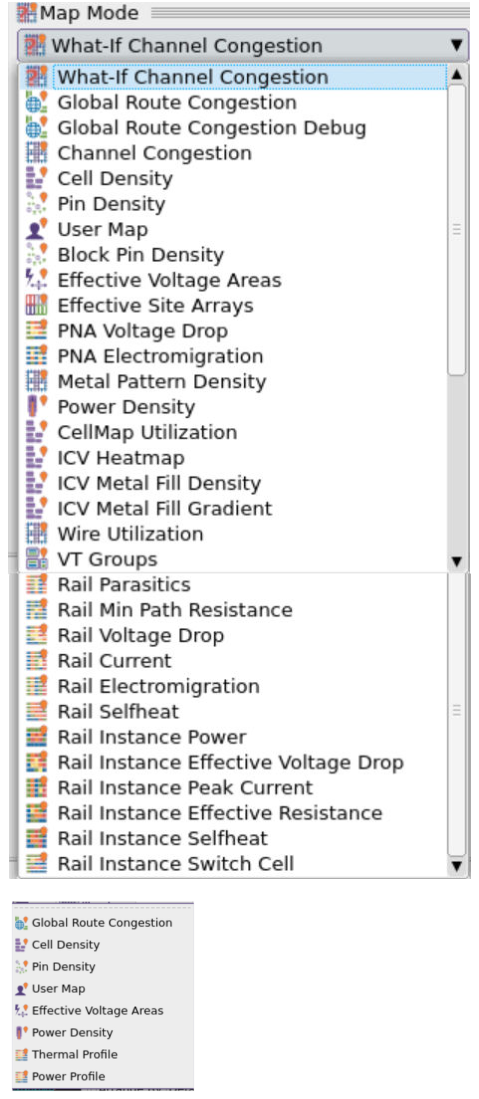
\includegraphics[width=0.92\textwidth]{gui-fig-093.png}
\caption{Map 模式}
\label{fig:gui-93}
\end{figure}

\begin{figure}[htbp]
\centering
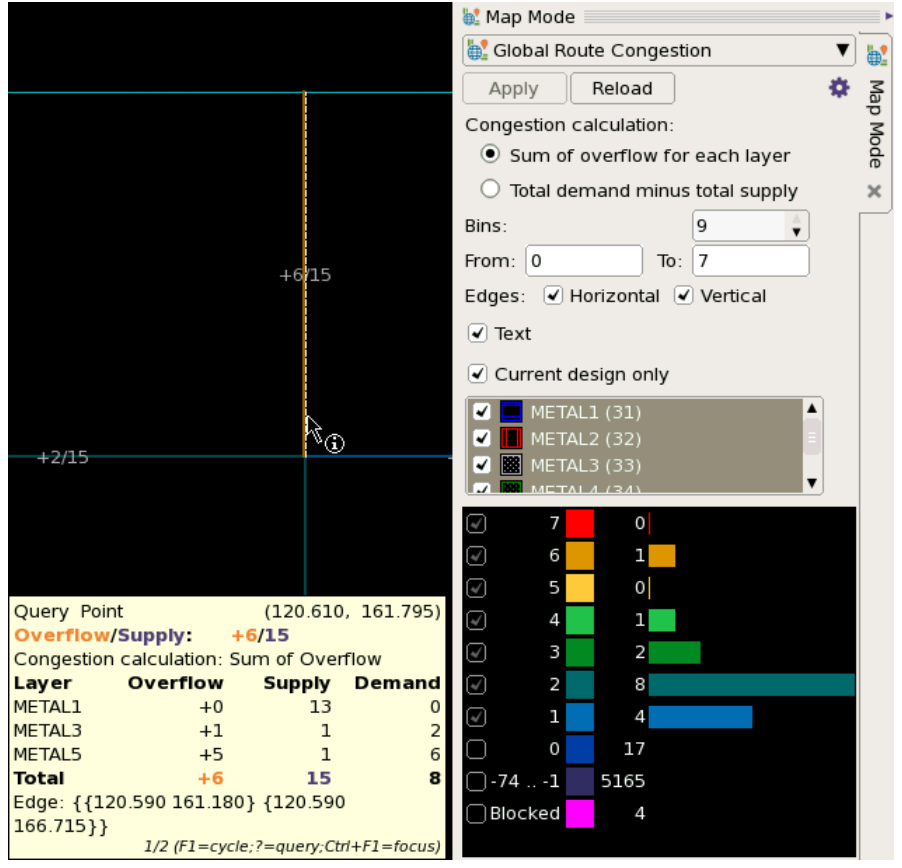
\includegraphics[width=0.92\textwidth]{gui-fig-094.png}
\caption{全局布线拥塞图}
\label{fig:gui-94}
\end{figure}

\subsection{配置直方图}
\subsubsection*{Configuring the Histogram}

在 map mode 面板底部，工具显示当前 map mode 的数值直方图（histogram）。首次生成直方图时必须单击 Reload。要修改直方图：
\begin{itemize}
  \item 选中或取消条形左侧的复选框，即可在版图中显示或隐藏直方图条及其对应数据；也可以在该行任意位置右键，选择 Show 或 Hide。还可以选择 Show all 或 Hide all，以显示或隐藏全部直方图条。
  \item 在该行任意位置右键并选择 Set Style，可更改直方图条以及版图中对应网格的颜色。
  \item 在该行任意位置右键并选择 Configure，可更改其他显示选项；详见「配置 Map 选项」。
\end{itemize}

单击 Apply，按新设置更新 map。

\begin{itemize}
  \item 选择 Show in List，并在 Map Data 对话框中单击某一行，即可定位到设计版图中的特定网格。
\end{itemize}

\begin{figure}[htbp]
\centering
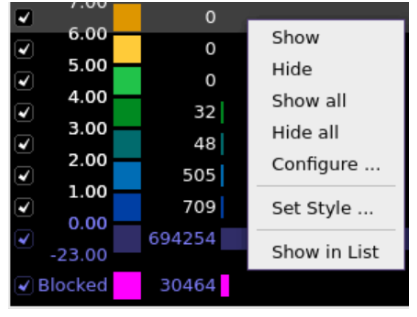
\includegraphics[width=0.92\textwidth]{gui-fig-095.png}
\caption{Map 模式直方图}
\label{fig:gui-95}
\end{figure}

\subsection{更改透明度}
\subsubsection*{Changing the Transparency}

可以用工具 GUI 中的 Alpha 控件调节 map 的透明度（transparency）。也可以对 \cmd{gui\_get\_map\_option}、\cmd{gui\_get\_map\_option\_list} 与 \cmd{gui\_set\_map\_option} 命令使用 \opt{-option} \cmd{alpha}。

下表说明部分设置如何影响 map 的透明度。

\begin{table}[htbp]
\centering
\caption{透明度控制设置}
\begin{tabularx}{\textwidth}{@{}l X@{}}
\toprule
Alpha 设置 & 透明度 \\
\midrule
100\% & 默认（Default），不透明（Opaque） \\
50\% & \\
Off & 完全透明（Fully transparent） \\
\bottomrule
\end{tabularx}
\end{table}

下面的例子用 \cmd{gui\_set\_map\_option} 命令设置透明度。
\begin{lstlisting}
icc2_shell> gui_set_map_option -map cellDensityMap -option alpha -value 10%
\end{lstlisting}

要取回设置，可以使用 \cmd{gui\_get\_map\_option} 命令。例如：
\begin{lstlisting}
icc2_shell> gui_get_map_option -map cellDensityMap -option alpha
\end{lstlisting}

\subsection{配置 Map 选项}
\subsubsection*{Configuring Map Options}

单击 Show Options 按钮并选择 configure，可以对每种 map mode 做进一步配置：
\begin{itemize}
  \item 夸张方案（exaggeration scheme）：设置 Top、Middle 与 Bottom 值，以指定 map mode 与 visual mode 中的颜色夸张方案。这些值设定在版图中显示拥塞条时使用的最小、中位与最大像素数。
  \item Show styles：显示或隐藏直方图中的色标方块。
  \item Show exaggeration：在每条直方图条旁显示或隐藏计算出的夸张值。
  \item Show counts：显示或隐藏每个直方图分档（bin）的边数。
  \item Show histogram：显示或隐藏直方图条。
  \item Show only visible bins in histogram：选中后，仅当该分档的复选框被选中时才显示对应的直方图条。
\end{itemize}

\section{全局布线拥塞图}
\subsection*{Global Route Congestion Map}

IC Compiler II 支持全局布线拥塞图（Global Route Congestion map），用来突出设计中对全局布线（global route）需求很高的区域。拥塞（congestion）区域可能在详细布线（detail route）期间引发问题。要显示全局布线拥塞图，选择 \textbf{View > Map > Global Route Congestion}，或单击 Global Route Congestion 按钮。

要生成全局布线拥塞图，单击 Reload 按钮。工具会显示一个对话框，其中给出用于生成 map 数据的 \cmd{route\_global} 命令及其选项。单击 OK 运行该命令。完成后，工具显示拥塞图。

工具显示拥塞图之后，把指针移到版图窗口并放大，以便更细致地查看 map。把指针移到拥塞条上，可在信息提示（infotip）中查看更多信息。

\subsection{细化全局布线拥塞图}
\subsubsection*{Refining the Global Route Congestion Map}

可以修改 Global Route Congestion Map 面板中的设置，以改变拥塞图的显示方式。使用下列设置更改拥塞图：
\begin{itemize}
  \item Rule level：选择拥塞计算所采用的规则级别。
  \item Congestion calculation：选择 Sum of overflow for each layer 或 Total demand minus total supply，以指定计算拥塞的方法。该设置如何影响显示，见「拥塞图计算」。
  \item Bins：更改 Bins 的值，以改变显示 map 所用的唯一分档数目。分档越多，map 被划分成的取值范围就越多。
  \item From: 与 To:：更改这两个值，以改变 map 与直方图中显示的溢出（overflow）值范围。这些值表示布线单元（route cell）上布线容量的溢出，数值越大表示拥塞越严重。
  \item Edges：选择要显示拥塞值的全局布线单元（global route cell）的边，即 Horizontal 与 Vertical。
  \item Text：选择此项后，在版图中显示一个代表计算出的拥塞值的数字。若看不到这些值，必须放大查看，并确认直方图中已选中相应范围。
  \item Hierarchical：选择此项后，在层次块内部显示拥塞图。
  \item Layers：选择计算拥塞时要考虑的布线层。
\end{itemize}

在面板底部，工具显示拥塞值的直方图。生成 map 之后，可以这样修改直方图：
\begin{itemize}
  \item 选中或取消各层，使它们纳入或排除在拥塞计算之外。
  \item 选中或取消条形左侧的复选框，以在版图中显示或隐藏直方图条及其对应网格；也可以在该行任意位置右键，选择 Show chosen rows 或 Hide chosen rows。
  \item 在该行任意位置右键并选择 Set Style，可更改直方图条以及版图中对应网格的颜色。
  \item 单击 Apply，按新设置更新 map。
\end{itemize}

\subsection{拥塞图计算}
\subsubsection*{Congestion Map Calculations}

全局布线拥塞图支持两种计算模式：“Sum of overflow for each layer”与“Total demand minus total supply”。当某个全局布线单元存在拥塞时，模式决定工具显示的拥塞值。默认模式是各层溢出求和。

下面给出两种模式的计算示例。该示例说明拥塞设计中穿过一个全局布线单元的一个方向。

\begin{figure}[htbp]
\centering
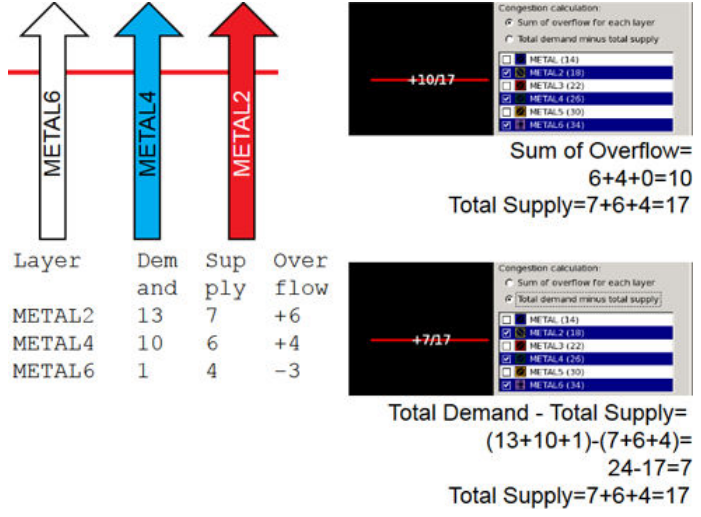
\includegraphics[width=0.92\textwidth]{gui-fig-096.png}
\caption{拥塞示例}
\label{fig:gui-96}
\end{figure}

在本例中，层 METAL2 严重拥塞：布线轨道的需求（demand）为 13，供给（supply）只有 7，溢出为 6。层 METAL4 中等拥塞，溢出为 4。层 METAL6 没有拥塞，下溢（underflow）为 3。本例中其他层不参与拥塞计算。

各层溢出求和是默认计算模式，只考虑每一层的溢出。本例中 METAL2 的溢出为 6，METAL4 的溢出为 4，溢出总和为 $6+4=10$。METAL6 上没有溢出，因此即使选中了该层，也不参与计算。在只含下溢的区域中，工具对每个被选中的层的下溢求和。

Total Demand Minus Total Supply 计算把总需求相加，再减去总供给。本例中总需求为 24，总供给为 17，结果为 $24-17=7$。请注意，在同时含有溢出与下溢的区域中，Total Demand Minus Total Supply 会给出更乐观的拥塞结果。

\subsection{检查拥塞区域中的单元}
\subsubsection*{Examining Cells in Congested Areas}

当拥塞图可见时，可以用拥塞区域对话框在版图视图中定义一个矩形区域，从而查看并选择设计中跨多层的拥塞区域内的单元。对话框列出该区域内拥塞区域中的单元。

可以在单元列表中选择单元，以便在版图视图中查看或高亮它们，也可以设置最小全局布线拥塞（global routing congestion，GRC）违例阈值来过滤单元列表。此外，可以对拥塞区域中的单元做交叉探测（cross-probe），定位到寄存器传输级（register-transfer level，RTL），从而找出可能导致拥塞的 RTL 代码。

要选择并查看拥塞区域中的单元：
\begin{enumerate}
  \item （可选）若只想查看顶层层次上的拥塞区域，选中 “Current design only” 复选框。

  若未选中该复选框（这是默认情况），则显示跨越物理层次的拥塞区域。
  \item 在 Global Route Congestion 面板上单击 “Cells in congested region” 按钮。

  出现拥塞区域对话框。可以把该对话框移到屏幕上某个位置，以便同时使用对话框和版图视图。
  \item 用下列方式之一定义区域的形状与位置：
  \begin{itemize}
    \item 在版图视图中拖动指针，在需要的位置形成矩形；
    \item 或在 “GR Congestion region” 框中输入矩形左上角与右下角的 $x$ 与 $y$ 坐标。
  \end{itemize}
  \item 单击 Apply。

  区域内的单元名称出现在 Cell Name 列表中。列表中只包含高度拥塞区域内的单元。
  \item （可选）要按全局布线拥塞阈值过滤单元，在 “GRC violation threshold” 框中输入一个值。

  只有全局布线阈值大于或等于该值的单元才会出现在对话框中。
  \item 若需要列出设计中另一区域的单元，重复第 2 步到第 4 步。
\end{enumerate}

单元列表树有两种模式：File/Line/Object 与 File/Object。File/Line/Object 模式显示每个文件每一行上的对象。File/Object 模式显示每个文件的对象。

要在版图视图中选择并查看拥塞单元，在单元列表中选择单元名称。版图视图以选择色显示这些选中的单元，选择色默认为白色。

\subsection{交叉探测拥塞区域中的单元}
\subsubsection*{Cross-Probing Cells in Congested Areas}

在拥塞分析期间，对高度拥塞区域中的单元做交叉探测，有助于找出引起拥塞的 RTL 代码。

要快速查看某个单元的 RTL，在 Cells in Congested Region 面板中单击该单元。RTL 代码会在 RTL 浏览器中高亮。

\section{通道拥塞图}
\subsection*{Channel Congestion Map}

通道拥塞图（Channel Congestion map）显示对象之间的通道（channel）中对全局布线需求很高的设计区域。可以为设计中的一小块区域生成通道拥塞图，修改设计后再重新生成 map，以便快速迭代、修复设计中的拥塞区域。要显示全局布线拥塞图，选择 \textbf{View > Map > Global Route Congestion}，或单击 Global Route Congestion 按钮。

要生成通道拥塞图，单击 Reload 按钮。工具显示一个对话框；选择 Whole design area 或 Specified area，以定义要分析通道拥塞的区域。单击 OK 运行命令。完成后，工具显示通道拥塞图。

工具显示通道拥塞图之后，把指针移到版图窗口并放大，以便更细致地查看 map。把指针移到拥塞条上，可在信息提示中查看更多信息。

可以修改 Channel Congestion Map 面板中的设置，以改变拥塞图的显示方式。按下列各项更改拥塞图：
\begin{itemize}
  \item Congestion calculation：选择 Sum of overflow for each layer 或 Total demand minus total supply，以指定计算拥塞的方法。该设置如何影响显示，见「拥塞图计算」。
  \item Bins：更改 Bins 的值，以改变显示 map 所用的唯一分档数目。分档越多，map 被划分成的取值范围就越多。
  \item From: 与 To:：更改这两个值，以改变 map 与直方图中显示的溢出值范围。这些值表示布线单元上布线容量的溢出，数值越大表示拥塞越严重。
  \item Edges：选择要显示拥塞值的全局布线单元的边，即 Horizontal 与 Vertical。
  \item Text：选择此项后，在版图中显示一个代表计算出的密度值的数字。若看不到这些值，必须放大才能查看。
  \item Hierarchical：选择此项后，在层次块内部显示拥塞图。
  \item Layers：选择计算拥塞时要考虑的布线层。
\end{itemize}

修改直方图的更多信息见「配置直方图」。

\section{单元、管脚、块管脚与功耗密度图}
\subsection*{Cell, Pin, Block Pin, and Power Density Maps}

密度图（density map）显示核区域（core area）内、或核内某一矩形区域中，某类对象或某个计算值的高密度（density）区域。IC Compiler II 提供单元密度图（Cell Density Map），用于分析标准单元（standard cell）的密度；提供管脚密度图（Pin Density Map），用于分析给定区域内管脚的密度；并提供功耗密度图（Power Density map），用于分析版图中的功耗密度。块管脚密度图（Block Pin Density map）显示块管脚边上的管脚密度。要显示相应的单元密度图：
\begin{itemize}
  \item 选择 \textbf{View > Map > Cell Density}，或单击 Cell Density 按钮，以显示单元密度图。
  \item 选择 \textbf{View > Map > Pin Density}，或单击 Pin Density 按钮，以显示管脚密度图。
  \item 选择 \textbf{View > Map > Block Pin Density}，或单击 Block Pin Density 按钮，以显示块管脚密度图。
  \item 选择 \textbf{View > Map > Power Density}，或单击 Power Density 按钮，以显示功耗密度图。
\end{itemize}

要生成 map，单击 Reload 按钮。工具显示一个对话框；选择 Whole design area 或 Specified area，以定义要分析的区域。单击 OK 运行命令。完成后，工具显示单元密度图。

工具显示 map 之后，把指针移到版图窗口并放大，以便更细致地查看 map。把指针移到网格点上，可在信息提示中查看更多信息。对于单元密度图、管脚密度图与功耗密度图，Grid size 标签显示当前 map 中水平与垂直网格点的数目。Grid size 的值由每个网格点所含的标准单元高度数目，以及你指定的、用于计算 map 的矩形大小决定。

可以修改 map 面板中的下列设置，以改变显示：
\begin{itemize}
  \item Grid dimension：选择用来为单元密度图、管脚密度图或功耗密度图定义网格的标准单元高度数目。
  \item Solid filled grids：对单元密度图、管脚密度图或功耗密度图，用代表该段版图密度的直方图颜色填充每个网格单元。
  \item Bins：更改 Bins 的值，以改变显示 map 所用的唯一分档数目。分档越多，map 被划分成的取值范围就越多。
  \item From: 与 To:：设置单元密度图、管脚密度图或功耗密度图中显示的密度值范围。
  \item Text：在版图中显示一个数字，表示每个网格点上计算出的密度值。若看不到这些值，必须放大才能查看。
  \item Current design only：只为当前层次级别显示密度图。
\end{itemize}

修改直方图的更多信息见「配置直方图」。

\section{有效电压区域图}
\subsection*{Effective Voltage Areas Map}

有效电压区域图（Effective Voltage Areas map）显示设计的默认电压区域（voltage area）以及其他由用户创建的电压区域。要显示有效电压区域图，选择 \textbf{View > Map > Effective Voltage Areas}，或单击 Effective Voltage Areas 按钮。

工具显示 map 之后，把指针移到某个电压区域上，可在信息提示中查看更多信息。单击该电压区域，即可在 Query 面板中显示有关该电压区域的信息。

可以修改 Effective Voltage Areas map 面板中的设置，以改变 map 的显示方式。按下列各项更改 map 显示：
\begin{itemize}
  \item Show as fractured rectangles：选择此项，把电压区域显示为碎裂矩形（fractured rectangle）。
  \item Hierarchical：选择此项，在层次块内部显示管脚密度图。
\end{itemize}

修改直方图的更多信息见「配置直方图」。

\section{有效站点阵列图}
\subsection*{Effective Site Arrays Map}

有效站点阵列图（Effective Site Arrays map）显示设计中当前已定义的站点阵列（site array）。要显示有效站点阵列图，选择 \textbf{View > Map > Effective Site Arrays}，或单击 Effective Site Arrays 按钮。

工具显示 map 之后，把指针移到站点阵列上，可在信息提示中查看更多信息。单击该站点阵列，即可在 Query 面板中显示有关该站点阵列的信息。

选择 Current design only 选项，则只显示当前层次级别的站点阵列。

修改直方图的更多信息见「配置直方图」。

\section{线利用率图}
\subsection*{Wire Utilization Map}

线利用率图（Wire Utilization map）在版图上显示利用率（utilization）数值。利用率是布线轨道需求除以容量；其中需求是被预布线（preroute）与详细布线图形（detail route shape）占用的轨道数。

要显示线利用率图，从菜单选择 \textbf{View > Map > Wire Utilization}。线利用率图见图~\ref{fig:gui-97}。

\begin{figure}[htbp]
\centering
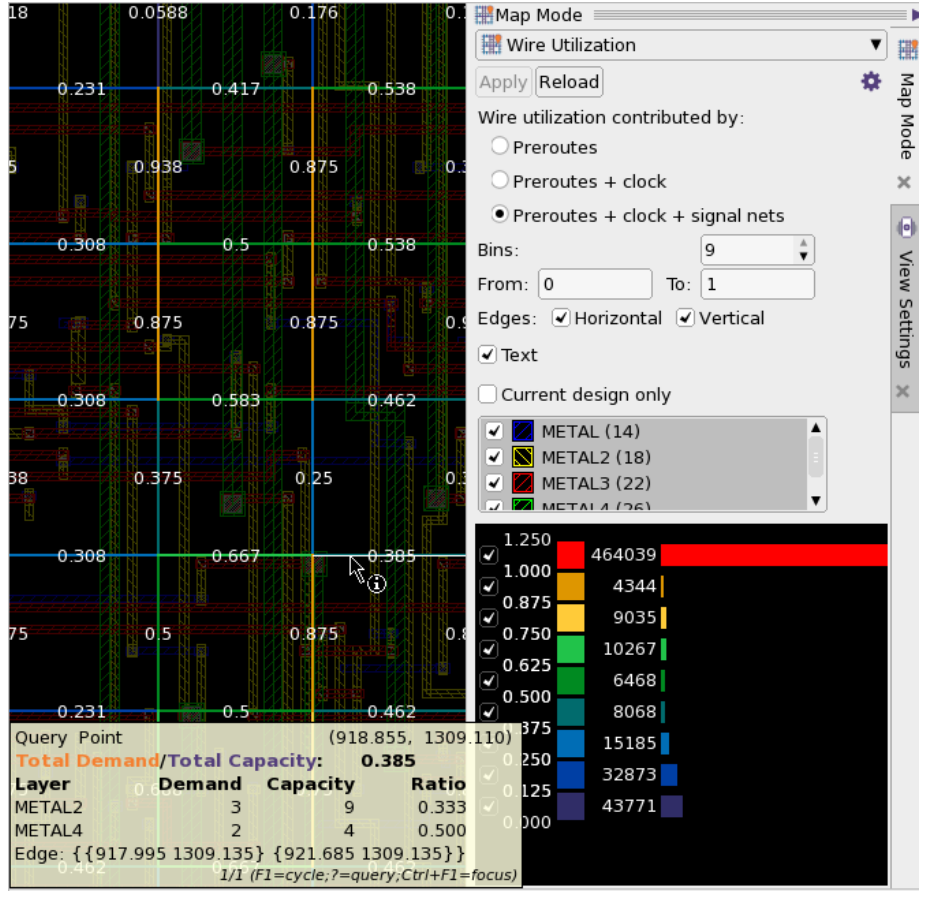
\includegraphics[width=0.92\textwidth]{gui-fig-097.png}
\caption{线利用率图}
\label{fig:gui-97}
\end{figure}

修改 Wire Utilization map 中的设置，以改变 map 的显示方式：
\begin{itemize}
  \item Wire utilization contributed by：选择 Preroutes、Preroutes + clock，或 Preroutes + clock + signal nets。计算需求数时只计入所选的布线类型。
  \item Bins：更改 Bins 的值，以改变显示 map 所用的唯一分档数目。分档越多，map 被划分成的取值范围就越多。
  \item From: 与 To:：更改这两个值，以改变 map 与直方图中显示的溢出值范围。这些值表示布线单元的利用率。
  \item Edges：选择要显示利用率值的边，可以是 Horizontal、Vertical，或两者都选。
  \item Text：在版图中显示一个代表计算出的利用率值的数字。若看不到这些值，必须放大才能查看。
  \item Current design only：把利用率计算限制在当前层次级别。
  \item Layers：选择计算利用率时要考虑的布线层。
\end{itemize}

修改直方图的更多信息见「配置直方图」。

\section{导出与导入 Map 数据}
\subsection*{Exporting and Importing Map Data}

工具支持读取与写出 map 数据。

该功能使你可以：
\begin{itemize}
  \item 以简单的 ASCII 格式导出 map 数据。你可以后处理该 ASCII 文件，或把它作为其他工具的输入。
  \item 把 map 数据导入（或读入）工具，并用 User Map 这一 map mode 生成图或直方图。
\end{itemize}

工具以简单 ASCII 格式读写 map 数据。该格式包含下列部分：元数据（metadata，可选）、表头（header，可选）以及数据。对于可选部分，若未作任何指定，会自动套用默认值。下面是 map 数据文件可能的样子。
% 提取文本在此句之后未保留示例文件正文。

要导出某个特定 map 的 map 数据：
\begin{enumerate}
  \item 在 GUI 中，于版图视图里启用一种 map mode，例如全局布线拥塞图。
  \item 单击 Settings 图标。
  \item 选择 Export as User Map file。
  \item 在 \cmd{gui\_write\_user\_map} 对话框中输入文件名。
  \item 单击 OK。
\end{enumerate}

输出文件以 CSV 格式包含 map 数据。

\begin{noteBox}
输出文件包含整个设计区域的数据，而不是所选区域的数据。工具会忽略未被选中的层。
\end{noteBox}

对于元数据与表头部分中为空的值，工具会自动填入默认值。

{\small
\setlength{\tabcolsep}{3pt}
\begin{longtable}{@{}p{1.05cm}p{0.7cm}p{2.15cm}p{2.55cm}p{1.7cm}p{3.55cm}p{2.15cm}@{}}
\caption{Map 数据 ASCII 文件的元数据默认值}\\
\toprule
类型 & 名称 & 属性 & 值 & 默认值 & 说明 & 示例 \\
\midrule
\endfirsthead
\caption{Map 数据 ASCII 文件的元数据默认值（续）}\\
\toprule
类型 & 名称 & 属性 & 值 & 默认值 & 说明 & 示例 \\
\midrule
\endhead
table & “” & \cmd{app\_name} & string & “” & 用于写出 map 数据的工具 & fc \\
table & “” & \cmd{report\_date} & string & “” & 生成 map 数据的日期与时间 & 2020-Sep-30 09:49:58 \\
table & “” & \cmd{title} & string & \cmd{map\_filename} & Map 标题 & Cell Density \\
table & “” & \cmd{version} & string & “” & 用户 map 版本 & V 1.0 \\
table & “” & \cmd{bins} & int & 10 & Map 的分档计数 & 9 \\
table & “” & \cmd{max\_threshold} & int 或 float & “” & 最大 map 数据 & 1.0 \\
table & “” & \cmd{min\_threshold} & int 或 float & & 最小 map 数据 & 1.0 \\
table & “” & \cmd{color\_scale} & TemperatureScale/RainbowScale/QualitativeScale & TemperatureScale & 三套配色方案，工具按分档数目设置 & TemperatureScale \\
\bottomrule
\end{longtable}
\setlength{\tabcolsep}{6pt}
}

{\small
\setlength{\tabcolsep}{3pt}
\begin{longtable}{@{}p{1.5cm}p{2.6cm}p{1.8cm}p{2.2cm}p{6.2cm}@{}}
\caption{Map 数据 ASCII 文件的表头默认值}\\
\toprule
类型 & 名称 & 属性 & 值 & 说明 \\
\midrule
\endfirsthead
\caption{Map 数据 ASCII 文件的表头默认值（续）}\\
\toprule
类型 & 名称 & 属性 & 值 & 说明 \\
\midrule
\endhead
column & Coordinates type & \cmd{poly\_rect} & &
map 数据的区域，可以是多边形或矩形。矩形的坐标格式为 \cmd{\{llx lly\} \{urx ury\}}（默认）或 \cmd{llx lly urx ury}。例如 \cmd{\{10 10\} \{50 50\}} 或 \cmd{10 10 10 50}。多边形的坐标格式为 \cmd{\{x1 y1\} \{x2 y2\} \ldots\ \{xn yn\}} 或 \cmd{x1 y1 x2 y2 \ldots\ xn yn}，其中 $x_1=x_n$ 且 $y_1=y_n$。例如 \cmd{\{20 20\} \{20 40\} \{30 40\} \{30 30\} \{40 30\} \{40 20\} \{20 20\}} 或 \cmd{20 20 20 40 30 40 30 30 40 30 40 20 20 20}。 \\
column & Value & type & int 或 float & 数据。示例值为 0.835556。 \\
column & Comment & type & string &
数据的文本信息。对于在版图视图中显示对象的 map，注释为对象名。例如 “map\_data: 0.83556”。 \\
column & Comment\_1 & type & string &
可选注释，用来表明数据位于特殊分档中。例如布线拥塞图中的被阻塞区域。 \\
\ldots & \ldots & type & string &
你希望添加的可选注释。其他附加列。 \\
\bottomrule
\end{longtable}
\setlength{\tabcolsep}{6pt}
}

在把 map 数据导入工具之前，可以先预览。

你可能希望在把 map 数据载入工具之前，确认这些数据是准确的。GUI 提供预览对话框，用来预览 map 数据。

要预览 map 数据：
\begin{enumerate}
  \item 确认 map 数据已保存为 CSV 文件。

  关于如何生成 CSV 文件，见「要导出某个特定 map 的 map 数据」。
  \item 使用 \opt{-preview} 选项运行下列命令：
\begin{lstlisting}
icc2_shell> gui_read_user_map -preview -file global_congestion.csv
\end{lstlisting}
  在本例中，\cmd{global\_congestion.csv} 与设计位于同一目录。若文件在其他位置，请给出文件路径。

  出现 (Re)Load User Map Data 对话框，其中的 Column、Base Type、Data Type 与 First Row Values 由 CSV 文件填入。若有错误，对话框会显示这些错误。
  \item （可选）在 CSV 文件中改正错误，并在导入之前预览数据。

  也可以使用 User Map 调色板中的 Reload 按钮来打开预览对话框。
\end{enumerate}

要导入 map 数据：
\begin{enumerate}
  \item 在 GUI 中，于版图视图里启用 User Map 这一 map mode：\textbf{View > Map > User Map}。
  \item 单击 Reload。
  \item 在 (Re)Load User Map Data 对话框中，输入 CSV 文件的名称（含完整路径）。

  载入数据可能需要几分钟。
\end{enumerate}

数据载入完成后，版图视图显示 map 数据。例如：

要把已从文件读入的 map 数据从版图视图中去掉：
\begin{enumerate}
  \item 在 GUI 中，于版图视图里启用 User Map 这一 map mode：\textbf{View > Map > User Map}。
  \item 单击 Remove Current Map。
\end{enumerate}
